\section*{Theory}

\subsection*{k-Space-Domain Subproblems}
We propose to compute a sparse 
design matrix $\bm{W}$ that directly maps the Fourier transform of a desired spatial 
excitation pattern to a vector of RF pulses that together produce the pattern, as:
\begin{equation}
\bm{b} = \bm{W} \mathcal{F}(\bm{d}),
\end{equation}
where $\bm{b}$ is a vector of concatenated multi-channel RF pulses with length $N_t  N_c$, 
where $N_t$ and $N_c$ are the numbers of time points and channels, respectively,
and $\mathcal{F}(\bm{d})$ is a length-$N_s$ vector containing the 
Fourier transform of the desired k-space excitation pattern $\bm{d}$.
$\bm{W}$ has dimensions $N_t  N_c \times N_s$.
Once the entries of $\bm{W}$ are computed, 
the RF design problem can be instantaneously solved by a sparse matrix multiplication, 
without a full matrix inversion or an iterative algorithm. 
Here we describe how to break down the problem of constructing $\bm{W}$ 
into a set of smaller independent subproblems that can be solved in parallel. 

%Furthermore, in design problems involved iterative procedures, such as the phase updates in magnitude-least-squares pulse designs \cite{setsompop2008magnitude} and the regularization factor updates in power/roughness constrained pulse design, the sparsity of the $\bm{W}$ matrix makes the iterative process much more efficient in terms of memory and speed. In the work of Katscher et al \cite{katscher2003transmit}, parallel transmit pulse design was also formulated in the k-space domain. However, in Ref \cite{katscher2003transmit}, the matrix $\bm{W}$ was solved as a whole, which required constructing and inverting a large $\bm{S}^H\bm{S}$ matrix, which will be explained in the following text. Our proposed method finely divides the process of finding $\bm{W}$ into many independent instances, which allows the use of parallel computing to largely accelerate the computation. Furthermore, the $\bm{S}^H\bm{S}$ matrices of different instances are each small, and our proposed method efficiently constructs these matrices, which further accelerates the computation. 

\par The columns of $\bm{W}$ can be solved independently, 
based on the observation that if the desired k-space pattern is a delta function at a k-space location 
$\vec{k}_j$ ($1\leq j \leq N_s$), 
then only the $j$-th column $\bm{w}_j$ of $\bm{W}$ is required to relate 
the desired k-space pattern to the desired RF pulse. 
In this case, the vector $\bm{w}_j$ is identical to the desired RF. 
Therefore, the problem of finding the $j$-th column $\bm{w}_j$ of $\bm{W}$ can be restated as: 
what should the RF pulse samples be to generate a unit delta function at the location $\vec{k}_j$ in k-space, 
and zeros elsewhere? 
Mathematically, the relationship that should be satisfied by the weights in column $\bm{w}_j$  can be expressed as:   
\begin{equation}\label{eq:ScalerForm}
\delta(\vec{k}-\vec{k}_j)=\sum_{i=1}^{N_t}\sum_{c=1}^{N_c} w_c(\vec{k}_i) s_c(\vec{k}-\vec{k}_i)
\end{equation}
where $i$ indexes time points in the pulses' excitation k-space trajectory, 
and $c$ indexes channels. 
$w_c(\vec{k}_i)$ is the $((c-1)N_t+i)$-th element of the $\bm{w}_j$ vector,
and $s_c(\vec{k}-\vec{k}_i)$ is the Fourier transform of channel-$c$'s $B_1^+$ map, 
shifted to be centered at excitation k-space location $\vec{k}_i$. 
Equation \ref{eq:ScalerForm} can be restated in matrix-vector form as:                                       
\begin{equation}\label{eq:MatrixForm}
\bm{Sw}_j=\bm{\delta}_j,
\end{equation}
where $\bm{S}$ is a $N_s \times N_c  N_t$ 
matrix containing values of $s_c(\vec{k}-\vec{k}_i)$ for all $c$ and $i$,
and $\bm{\delta}_j$ is a vector containing a one in the entry corresponding to excitation k-space location
$\vec{k}_j$, and zeros in all other entries. 
The regularized pseudoinverse solution for $\bm{w}_j$ is:                      
\begin{equation}\label{eq:Solution}
\bm{w}_j=\left( \bm{S}^{H} \bm{S} + \lambda \bm{I} \right) ^{-1} \bm{s}_j^{H}
\end{equation}
where $\bm{s}_j^{H}$ is the conjugate transpose of the $j$-th row of $\bm{S}$. 

\par If all points on the excitation k-space trajectory are considered in Equation \ref{eq:ScalerForm},
then there is no reduction in computation compared to a conventional pseudoinverse-based pulse design.
However, because $B_1^+$ maps are compact in excitation k-space and localized near DC,
only a small number ($\ll N_t$) of trajectory points near the target location $\vec{k}_j$ can contribute significantly
to the excitation pattern at $\vec{k}_j$ or its neighbors, 
and therefore need to be considered in the subproblem;
all other trajectory points can be ignored.
This means we can modify Equation \ref{eq:ScalerForm} to:
\begin{equation}
\delta(\vec{k}-\vec{k}_j) = \sum_{\vec{k}_i \in \mathbb{N}}\sum_{c=1}^{N_c} w_c(\vec{k}_i) s_c(\vec{k}-\vec{k}_i),
\end{equation} 
where $\mathbb{N}$ is the set of trajectory points in the vicinity of $\vec{k}_j$. 
In this work we define `inclusion width' as the distance, 
in cycles per excitation field-of-view (cycles/FOV), 
from each target location $\vec{k}_j$ within which which all trajectory points are accrued into $\mathbb{N}$.
This reduced set of trajectory points reduces the column dimension of $\bm{S}$
and both dimensions of $\bm{S}^H\bm{S}$,
and implies that the design matrix $\bm{W}$ is sparse.
Figure \ref{fig:Patch}a illustrates a target point $\vec{k}_j$ for a two-dimensional spiral pulse design, 
and the nearby points on the spiral trajectory that need to be included in the solution for $\bm{w}_j$
for an inclusion width of 4 cycles/FOV.

%\par A key advantage of the proposed pulse design formalism is that it can be finely parallelized
%across the columns of the $\bm{W}$ matrix. 
\par The $\bm{W}$ matrix columns $\bm{w}_j$ can be solved in parallel one-at-a-time or patch-wise, 
wherein all target points in a patch share the same $\bm{S}^{H}\bm{S}$ matrix,
and their $\bm{s}_j^H$ vectors are concatenated in the column dimension
to form a matrix in Equation \ref{eq:Solution}. 
An illustration of a $4 \times 4$ patch and its included trajectory points is shown in Figure \ref{fig:Patch}b,
for a two-dimensional spiral pulse design. 
The inclusion width is also 4 cycles/FOV from any target point in the patch, 
%we truncate the $B_1^+$ map Fourier transforms to zero outside a 4 by 4 cycle/FOV square centered at DC. 
so all the excitation trajectory points within a $12 \times 12$ cycles/FOV square are included in the calculation. 

%Since target locations that are distant to $\vec{k}_j$ can also be ignored,
%the row dimension of $\bm{S}$ is also reduced to the size of a smaller neighborhood immediately surrounding $\vec{k}_j$. 
%These reduced problem dimensions further imply that the design matrix $\bm{W}$ is sparse. 
%Figure \ref{fig:Patch}a illustrates a target point $\vec{k}_j$, 
%the nearby points on a spiral trajectory that need to be included in the solution for $\bm{w}_j$,
%and the neighboring target location points where a zero excitation must be enforced. 
%In the following, we define target and trajectory neighborhood sizes, 
%and describe an efficient method to construct the $\bm{S}^{H}\bm{S}$ matrices.

\begin{figure}
	\centering
	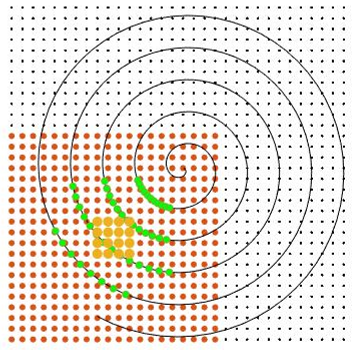
\includegraphics[width=6cm]{kspace_PTX_Patch}
	\caption{\textcolor{red}{WAG: I think you should make two subfigures here: one that illustrates a single target location, and one that illustrates a patch of target locations. Also you should annotate the different widths, in the figures, with arrows. Also add a legend for the dots} 
	Illustration of one instance within the palatalization of a 2D k-space domain design problem. The totally design problem is divided into patches of width 4 cycle/FOV, and the 16 yellow points are the target points in this instance. With inclusion width of 4 cycle/FOV, the 46 green excitation trajectory points within the 12 cycle/FOV wide green square (4 cycle/FOV extended outside of the patch) are considered in this instance. The excitation within the 20 cycle/FOV wide red patch is constrained to zero except the point where the delta function is.}
	\label{fig:Patch}
\end{figure}

\subsection*{Efficient $\bm{S}^H\bm{S}$ matrix construction}
%%which is 4 cycle/FOV extended outside of the patch width 4 square, since they may contribute energy to the target locations corresponding to the 16 $\bm{W}$ matrix columns. 
%For the patch illustrated in Figure \ref{fig:Patch}, 
%the 46 green points on the excitation trajectory may contribute significant energy and are considered in the weight design. 
%Furthermore, we must constrain the total excitation to zero at all k-space locations within a 20 by 20 cycle/FOV red patch in Figure \ref{fig:Patch}. 
%This is because any energy deposited at each considered excitation trajectory points will affect not only the target points in the yellow square, but also the whole 2$\times$4 wide patch around that trajectory point. And the 20 by 20 cycle/FOV red patch is the total of the points that can be affected by all the excitation trajectory points considered in this instance. Therefore, in the solution for this instance, $\bm{w}$ is a 46$N_c\times$16 matrix, $\bm{S}$ is a 400$N_c\times$46$N_c$ matrix, $\bm{S}^{H}\bm{S}$ is a 46$N_c\times$46$N_c$ matrix, and $\bm{s}_i^{H}$ is a 46$N_c\times$16 matrix. 
%%Since $\bm{s}_i^{H}$ is no longer related to the $i$th row of $\bm{S}$ and $i$th column of $\bm{W}$ only, it will be denoted as $\bm{S_{targ}}$ in later discussions. 
%In the next instance, another 16 columns centered around another 4 points by 4 points patch will be solved. It should be noted that in different instances, the number of neighboring excitation trajectory points (the 46 green points in the previous instance) can vary. We will denote this number of points by $N_n$. $N_n$ can be zero when a patch is at the corners where no excitation trajectory point is adjacent. 
%%For patches near edges of the excitation k-space FOV, the solution neighborhood and area may wrap back in a circulant shift fashion, depending on the resolution of the final spatial grid on which the user will evaluate the pulse. In Figure \ref{fig:Patch}), denoted by the red area to the right of Figure \ref{fig:Patch}).

%\par The patch width determines the total number of instances to be solved. The inclusion width determines the accuracy of $B_1^+$ information utilized in the design. Together, the patch width and the inclusion width determine how many excitation trajectory points are included in each instance, which further determines the size of $\bm{S}^{H}\bm{S}$ whose construction is most computationally burdensome within an instance. Therefore, increasing patch width reduces the number of $\bm{S}^{H}\bm{S}$ matrices to be constructed but increases the burden of constructing each of them. An optimal patch width should be decided case by case for different excitation trajectories. 

%\subsection*{Efficient construction of $\bm{S}^{H}\bm{S}$ matrix}
\par Constructing the $\bm{S}^{H}\bm{S}$ matrix by first constructing $\bm{S}$ is computationally expensive 
because it requires each channel's $B_1^+$ map to be shifted to each trajectory location $\vec{k}_i$
by phase modulation followed by Fourier transform, or by Fourier transform followed by interpolation. 
Furthermore, 
the matrix multiplication between $\bm{S}^{H}$ and $\bm{S}$ is also computationally intensive due to the potentially 
large row dimension of $\bm{S}$, if the zero excitation condition is enforced on a large grid of points around each $\vec{k}_j$.
The computational costs can be reduced by truncating the $B_1^+$ maps in k-space, 
but this introduces large errors. 
Instead, inspired by the rapid GRAPPA calibration method for arbitrary 2D/3D non-Cartesian trajectories of Ref \cite{luo2019grappa}, 
we propose to construct the Hermitian $\bm{S}^{H}\bm{S}$ matrix directly via interpolation of the Fourier transforms
of inner products of pairs of $B_1^+$ maps. 
The $\bm{S}^H\bm{S}$ matrix can be written in block form as:
\begin{equation}\label{eq:SHS_blocks}
\bm{S}^{H}\bm{S} = 
\begin{pmatrix}
\bm{S}_1^{H}\bm{S}_1 & \cdots & \bm{S}_1^{H}\bm{S}_{N_c} \\
\vdots  &  \ddots & \vdots  \\
\bm{S}_{N_c}^{H}\bm{S}_1 & \cdots & \bm{S}_{N_c}^{H}\bm{S}_{N_c} 
\end{pmatrix}, 
\end{equation}
where each sub-matrix $\bm{S}_i^H\bm{S}_j$ contains inner products of the Fourier transforms of channel $i$ and channel $j$'s 
$B_1^+$ maps, after they are shifted to be centered different points on the excitation trajectory corresponding to the row 
and column indices of the sub-matrix.
These inner products can be calculated by interpolating the Fourier transform of the inner product of 
channel $i$ and channel $j$'s $B_1^+$ maps. 
In other words, each element in the Hermitian matrix $\bm{S}_i^{H}\bm{S}_j$ 
is the vector sum of channel $i$ and channel $j$'s shifted k-space $B_1^+$ maps, 
which is also a single point of their k-space convolution. 
Via the multiplication property of the Fourier transform, 
this convolution in k-space can be calculated from the Fourier transform of the dot product of the two spatial domain $B_1^+$ maps. 
For further details, please refer to Ref. \cite{luo2019grappa}.
%In practice, $\bm{S}^{H}\bm{S}$ is constructed in the following way. 
%We first represent the $\bm{S}^{H}\bm{S}$ matrix with block matrices. Each block matrix $\bm{S}_i^{H}\bm{S}_j$ is of size $N_n$ by $N_n$, and $\bm{S}_i$ and $\bm{S}_j$ are the columns of $\bm{S}$ related to the k-space sensitivity maps of the $i$-th and $j$-th coils respectively.

\par Since $\bm{S}^{H}\bm{S}$ and its sub-matrices are Hermitian, 
we only need to find the values within the lower triangle of the matrix, 
which are the sub-matrices $\bm{S}_i^{H}\bm{S}_j$ with $i>j$ that are themselves lower triangular. 
The elements of a given sub-matrix $\bm{S}_i^{H}\bm{S}_j$ 
are interpolated from a densely sampled Fourier transform of the dot product of the spatial domain $B_1^+$ maps of the $i$-th and $j$-th channels. 
The $(m,n)$-th element is the value interpolated at a position $\vec{k}_m-\vec{k}_n$ away from DC,
where $\vec{k}_m$ and $\vec{k}_n$ are the excitation k-space trajectory locations corresponding to row $m$ and column $n$.
Compared to phase-modulating and Fourier transforming each channel's $B_1^+$ map for each point 
on the trajectory which would require $N_t  N_c$ Fourier transforms,
to solve all the columns of $\bm{W}$ the total number of Fourier transforms needed in this efficient method is $N_c(N_c+1)/2$. 
The storage size is also much smaller, 
and the potentially large matrix multiplication between $\bm{S}^H$ and $\bm{S}$ is avoided.
An alternative strategy would be to construct $\bm{S}$ by Fourier transforming each channel's $B_1^+$ map 
and then interpolating it to be centered at each trajectory location, 
but this again requires multiplication of the $\bm{S}^{H}$ and $\bm{S}$ matrices,
which further involves the multiplication of interpolated values. 
We have found empirically that this strategy introduces higher error
than interpolating the inner product values. 
%Furthermore, to calculate each element of $\bm{S}^{H}\bm{S}$, there are $2N_s$ number of interpolations involved with this sub-optimal strategy. While with the efficient algorithm there is only one interpolation from the densely sampled Fourier Transform of the dot product of two spatial domain $B_1^+$ maps needed. The extra interpolations involved in the sub-optimal strategy would introduce a larger error to $\bm{S}^{H}\bm{S}$.  

\subsection*{Off-Resonance Compensation}
% In order to model the off-resonance into our k-space domain design, we adapted a fast implementation of the off-resonance compensation with time segmentation approximation and weighted least-squares interpolators \cite{fessler2005toeplitz}. 
Off-resonance compensation is common in spatial-domain parallel pulse designs \cite{Grissom:2006:MRM}, 
but has not been previously implemented in a k-space-domain design.
Spatial domain designs based on non-uniform fast Fourier transforms make use of an approximate time-segmented
model for the off-resonance term \cite{fessler2005toeplitz},
which decouples the space- and time-dependence of off-resonant phase accrual into the product of 
space- and time-dependent terms, which are applied on either side of the non-uniform fast Fourier transform operator. 
Here we show that a time-segmented off-resonance model can be incorporated in the proposed k-space-domain algorithm. 
Mathematically, the time-segmented model is given by:
\begin{equation}
e^{\imath \Delta\omega_j (t_i-T) }\approx\sum_{l=1}^{L} g_l(t_i) e^{\imath \Delta\omega_j \breve{t}_l},
\end{equation}
where $\Delta\omega_j$ is the off-resonance frequency at location $\vec{x}_j$, 
$i$ indexes time points in the pulse, 
$T$ is the pulse duration,
and $l$ indexes the $L$ time segments, where $L$ is typically between 4 and 8. 
$g_{il}=b_{l}(t_i)$ are the temporal interpolators that multiply into the RF samples,
and $h_{lj}=e^{\imath \Delta\omega_j\breve{t}_l}$ are the off-resonance phase shifts 
applied to the excitation patterns produced by the RF pulse time segments centered at time points $\{\breve{t}_l: l = 1, \dots, L\}$.
We can incorporate the time-segmented off-resonance model into Equation \ref{eq:ScalerForm} as:
\begin{equation}
	\delta(\vec{k}-\vec{k}_j)=\sum_{l = 1}^L \sum_{i=1}^{N_t}\sum_{c=1}^{N_c} w_c(\vec{k}_i) g_l(t_i) \tilde{s}_{cl} (\vec{k}-\vec{k}_i), 
\end{equation}
where $\tilde{s}_{cl}(\vec{k})$ is the Fourier transform of the product of channel $c$'s $B_1^+$ map and time segment $l$'s 
off-resonance phase exponential. 
We can then write the equivalent of Equation \ref{eq:MatrixForm} with the off-resonance model:
\begin{equation}
	\sum_{l=1}^L \bm{S}_l \textrm{diag}(g_{il}) \bm{w}_j = \bm{\delta}_j,
\end{equation} 
where the matrix $\bm{S}_l$ is now formed from the $N_c  L$ Fourier transforms of the $B_1^+$ map and off-resonance
phase exponential products.  
Efficient construction of the $\bm{S}^{H}\bm{S}$ matrix follows much the same procedure as without
off-resonance except that with off-resonance,
the elements of each sub-matrix $\bm{S}_i^{H}\bm{S}_j$ in Equation \ref{eq:SHS_blocks}
are interpolated from $L(L+1)/2$ Fourier transformed maps,
and the interpolated values are weighted by the temporal interpolators for each pair of multiplied time segments before they 
are summed.
Compared to constructing $\bm{S}^H\bm{S}$ without off-resonance, 
taking off-resonance into account increases the total number of FFT operations form $N_c(N_c+1)/2$ to $N_cL(N_cL+1)/2$, 
and increases the number of interpolations needed for each sub-matrix element from 1 to $L(L+1)/2$.  
However, we note that only adjacent time segments with overlapping temporal interpolators at a given time point
need to be considered when calculating the elements of $\bm{S}^H\bm{S}$ corresponding to that time point. 



